\documentclass[aps,prl,5p,showpacs,showkeys,linenumbers, twocolumn]{revtex4-1}
\usepackage{hyperref}
\usepackage{graphicx}


\begin{document}
\title{Non-parabolicity and band gap renormalization in Si doped ZnO}
\author{R. E. Treharne}
\email[Corresponding Author: ]{R.Treharne@liverpool.ac.uk}
\affiliation{Stephenson Institute for Renewable Energy, University of Liverpool, UK}
\author{L. J. Phillips, K. Durose}
\affiliation{Stephenson Institute for Renewable Energy, University of Liverpool, UK}
\date{\today}
\begin{abstract}
\end{abstract}
\pacs{78.20.Jq, 88.66.sq, 81.15.-z}
\keywords{zinc oxide; magnetron sputtering; thin-film; doping; non-parabolicity, band gap normalisation}
\maketitle
\section{Introduction}



\section{Experimental Methods}

Films were deposited via RF magnetron sputtering using an AJA Phase II-J Orion system. The system was configured with a 'sputter-up' geometry with the substrate being suspended above two separate ceramic targets of ZnO and SiO$_2$ that were arranged off-centre and tilted at $5^{\circ}$ towards the middle of the substrate.  Soda-lime glass substrates (OptiWhite$^{TM}$, NSG) of size $100\times100\times4$ mm$^{3}$ were used throughout. They were cleaned by scrubbing with a nylon brush and a series of de-ionized water and isopropanol alcohol rinses followed by blow drying with a nitrogen gas jet. During deposition the ZnO and SiO$_2$ targets were sputtered from simultaneously using powers of $150$ W and $50$ W respectively. A growth pressure of 2mTorr Ar was used during deposition. The substrate temperature was maintained at $350\pm5^{\circ}$C during growth and the substrate was kept static (i.e was not rotated). Deliberate gradients of both thickness and composition were subsequently achieved across the resultant film to generate a `combinatorial' sample. A second film of pure SiO$_{2}$ was deposited under identical conditions (but without ZnO) to generate a reference film for calculating the \% wt. profile of SiO$_{2}$ in the co-sputtered film.

A Shimadzu UV-Vis-IR 3700 spectrophotometer with mapping capability was used to measure the transmittance of the co-sputtered film over the range 250 - 2500 nm. 289 spectra were taken in total at 5 mm increments over the full sample surface. At each of these 289 points the sheet resistance was also measured using a CMT-SR2000 4-point probe mapping system. Following transmittance and sheet resistance measurements the sample was cut into one hundred $10\times10$ mm$^2$ pieces. A selection of these pieces, 10 in total, were further scribed into four $5\times5$ mm$^2$ sections and Hall measurement were performed on each of these sections. The Hall measurement was performed with custom built equipment, provided by Semimetrics Ltd., using a field strength of 0.8 T.  Ellipsometry was performed on the same sections using a Woollam M2000-UI system. Ellipsometry was also used to map the thickness profile of the pure SiO$_{2}$ reference film.

\section{Results}

\section{Conclusions}

\begin{figure}[p]
\centering
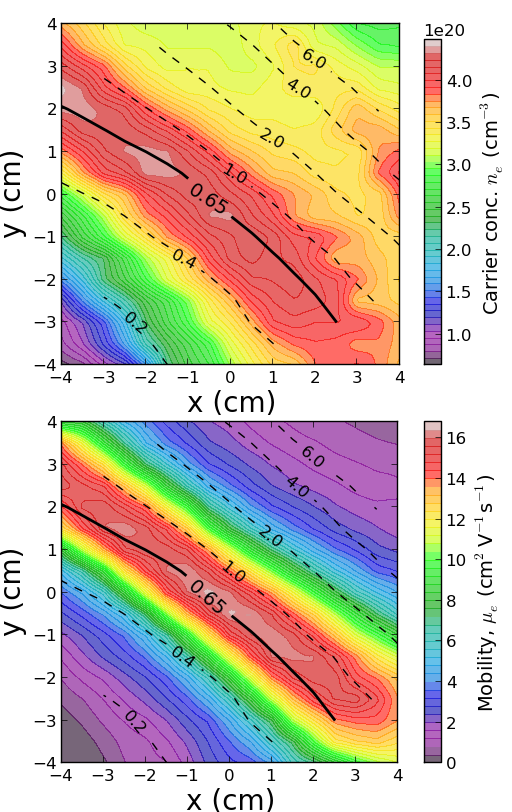
\includegraphics[width= \columnwidth]{figure2.png}
\caption{\label{fig:2} Contour maps of carrier concentration and mobility over the combinatorial sample. The (--) contour lines show an overlay of the \% wt. SiO$_{2}$ composition.}
\end{figure}

\begin{figure}[p]
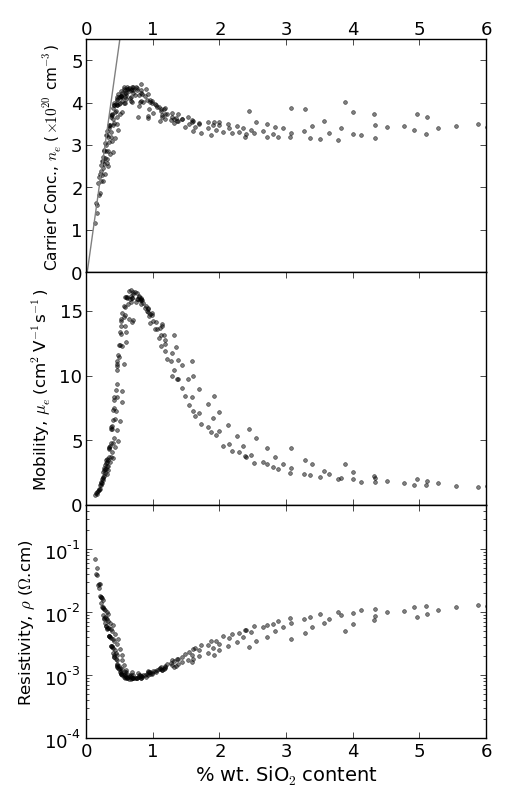
\includegraphics[width = 1\columnwidth]{figure3.png}
\caption{\label{fig:3} Distributions of carrier concentration, mobility and resistivity with respect to \% wt. SiO$_{2}$ content. The maximum values for $n_e$ ($4.4\times10^{20}$ cm$^{-3}$) and $\mu_{e}$ ($16.5$ cm$^{2}$V$^{-1}$s$^{-1}$) coincide with a composition of $0.65$\% wt. SiO$_{2}$. The solid straight line in the top plot shows the maximum theoretical carrier concentration with respect to SiO$_{2}$ content should every incorporated Si atom be substituted at a Zinc site and donate 2 carriers.}
\end{figure}

\begin{figure}[p]
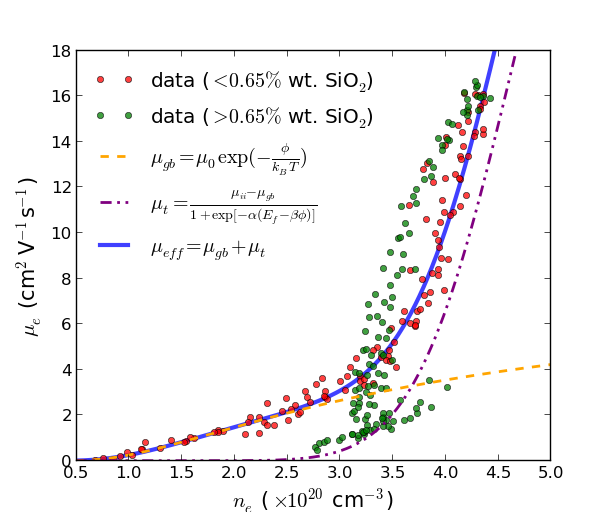
\includegraphics[width=1\columnwidth]{figure4.png}
\caption{\label{fig:4} }
\end{figure}

\begin{figure}[p]
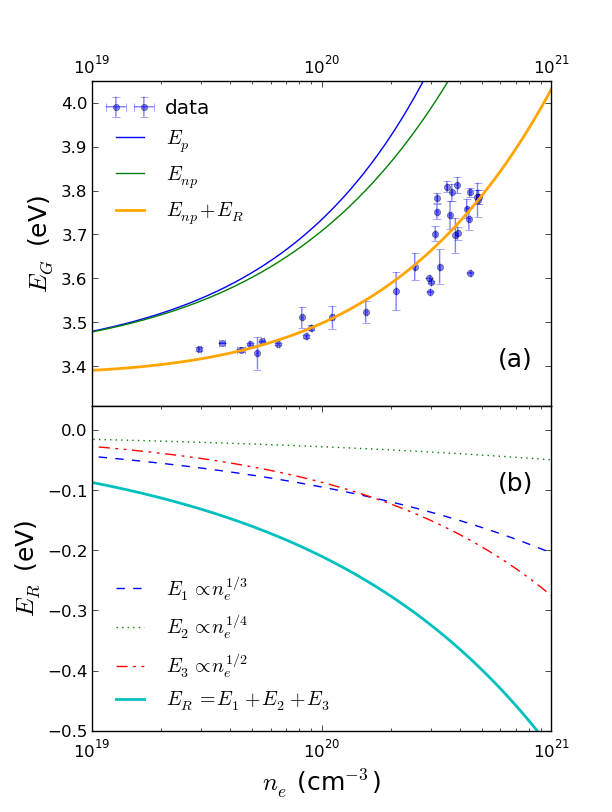
\includegraphics[width = 1\columnwidth]{figure5.png}
\end{figure}

\begin{acknowledgements}
The authors would like to thank ...
\end{acknowledgements}


\end{document}